\documentclass[12pt,a4paper]{article}
\usepackage[margin=1in]{geometry}
\usepackage{parskip}
\usepackage{microtype}
\usepackage{booktabs}
\usepackage{graphicx}
\usepackage{amsmath,amssymb}

\title{Alogos}
\author{Robin Langer}
\date{}

\begin{document}
\maketitle
\vspace{-1.5em}

\section{The name}

The Greeks called a number \emph{alogos} when it could not be written as a ratio of whole numbers. The word means \emph{without logos}, and logos means both \emph{ratio} and \emph{reason} --- the same word doing both jobs, because to them it was the same job. The Latin translators kept it exactly, and that is why we still say \emph{irrational}.

This document is about the machine for making such a number speak in ratios anyway, and about one quantity attached to that machine which turns out not to settle down.

\section{Continued fractions}

Let $x$ be a real number. Put
\[
  a_0 = \lfloor x \rfloor ,
\]
the largest whole number not exceeding $x$. If $x = a_0$ we are finished. Otherwise $x - a_0$ lies strictly between $0$ and $1$, so its reciprocal exceeds $1$; call it $x_1$, and we have
\[
  x \;=\; a_0 + \frac{1}{x_1}, \qquad x_1 > 1 .
\]
Now do the same to $x_1$: set $a_1 = \lfloor x_1 \rfloor$, and if $x_1 \neq a_1$ write $x_1 = a_1 + 1/x_2$. Repeating gives
\[
  x \;=\; a_0 + \cfrac{1}{a_1 + \cfrac{1}{a_2 + \cfrac{1}{a_3 + \cdots}}}
\]
which is abbreviated
\[
  x \;=\; [\,a_0;\ a_1, a_2, a_3, \ldots\,] .
\]
The whole numbers $a_i$ are the \emph{partial quotients}. Every $a_i$ with $i \geq 1$ is at least $1$, since each $x_i > 1$.

\textbf{The process stops exactly when $x$ is rational.} Running it on $x = p/q$ is Euclid's algorithm on the pair $(p,q)$, and Euclid's algorithm terminates. So a terminating continued fraction is a ratio, and a non-terminating one is not.

That is the sense in which the continued fraction answers the Greeks. An alogos number has no ratio, but it has an infinite sequence of them: truncating $[\,a_0; a_1, \ldots, a_i\,]$ gives an ordinary fraction $h_i/k_i$, the $i$-th \emph{convergent}, and these are in a precise sense the best rational approximations there are.

\section{Square roots repeat}

Take $x = \sqrt{n}$ for a whole number $n$ that is not a perfect square. The expansion never terminates, since $\sqrt n$ is irrational. What happens instead is that it \emph{repeats}.

\begin{center}
\begin{tabular}{ll}
\toprule
$\sqrt{2}$  & $[\,1;\ \overline{2}\,]$ \\
$\sqrt{3}$  & $[\,1;\ \overline{1,2}\,]$ \\
$\sqrt{5}$  & $[\,2;\ \overline{4}\,]$ \\
$\sqrt{6}$  & $[\,2;\ \overline{2,4}\,]$ \\
$\sqrt{7}$  & $[\,2;\ \overline{1,1,1,4}\,]$ \\
$\sqrt{13}$ & $[\,3;\ \overline{1,1,1,1,6}\,]$ \\
$\sqrt{19}$ & $[\,4;\ \overline{2,1,3,1,2,8}\,]$ \\
$\sqrt{31}$ & $[\,5;\ \overline{1,1,3,5,3,1,1,10}\,]$ \\
$\sqrt{94}$ & $[\,9;\ \overline{1,2,3,1,1,5,1,8,1,5,1,1,3,2,1,18}\,]$ \\
\bottomrule
\end{tabular}
\end{center}

The bar marks the block that repeats forever. Write
\[
  L(n) \;=\; \text{the length of that block.}
\]
So $L(2)=1$, $L(7)=4$, $L(94)=16$.

This is the whole subject of the document. $L(n)$ is a perfectly definite whole number, computable for any $n$ in a fraction of a second, and there is no formula for it. $L(61) = 11$ while $L(65) = 1$, and nothing about $61$ and $65$ explains the difference.

\section{Computing it}

The expansion of $\sqrt n$ can be generated without ever using a decimal. Keep a pair of whole numbers $(P_i, Q_i)$, starting from $a_0 = \lfloor \sqrt n \rfloor$, $P_0 = 0$, $Q_0 = 1$, and iterate
\[
  a_i = \left\lfloor \frac{a_0 + P_i}{Q_i} \right\rfloor,
  \qquad
  P_{i+1} = a_i Q_i - P_i,
  \qquad
  Q_{i+1} = \frac{n - P_{i+1}^{\,2}}{Q_i} .
\]
Every quantity here is an integer, and the division defining $Q_{i+1}$ is always exact. The block closes at the first $i \geq 1$ with $Q_i = 1$, and that index is $L(n)$.

Because nothing is approximated, there is no tolerance to choose and no error to accumulate. The values of $L(n)$ below are exact.

\section{Normalising}

$L(n)$ grows with $n$, roughly like $\sqrt n$, so comparing periods at different sizes means dividing that out. Put
\[
  t \;=\; \frac{L(n)}{\sqrt{n}} .
\]
Now fix a ceiling $M$ and collect $t$ for every non-square $n$ below it. That is a finite set of positive numbers, and we can ask what it looks like.

\section{The Weibull distribution}

To describe a positive quantity, write $S(t) = P(X > t)$ for the chance of exceeding $t$. The Weibull family is
\[
  S(t) \;=\; \exp\!\left(-\left(\frac{t}{\lambda}\right)^{\!k}\right),
  \qquad k > 0, \ \lambda > 0 .
\]
The scale $\lambda$ sets the units. The shape $k$ is the parameter of interest, and its meaning is clearest in the \emph{hazard} $h(t) = f(t)/S(t)$, the rate of stopping given that one has got as far as $t$:
\[
  h(t) \;=\; \frac{k}{\lambda}\left(\frac{t}{\lambda}\right)^{k-1} .
\]
So a Weibull is exactly a distribution whose hazard is a power of $t$, and $k$ is that power. If $k > 1$ the hazard rises; if $k < 1$ it falls; and $k = 1$ is the flat, memoryless case.

Given data, $k$ and $\lambda$ are chosen by maximum likelihood.

\section{The density, for small ceilings}

Below are the collected values of $t = L(n)/\sqrt n$ for four small ceilings, each with the Weibull of best fit drawn over it and its shape recorded.

\begin{center}
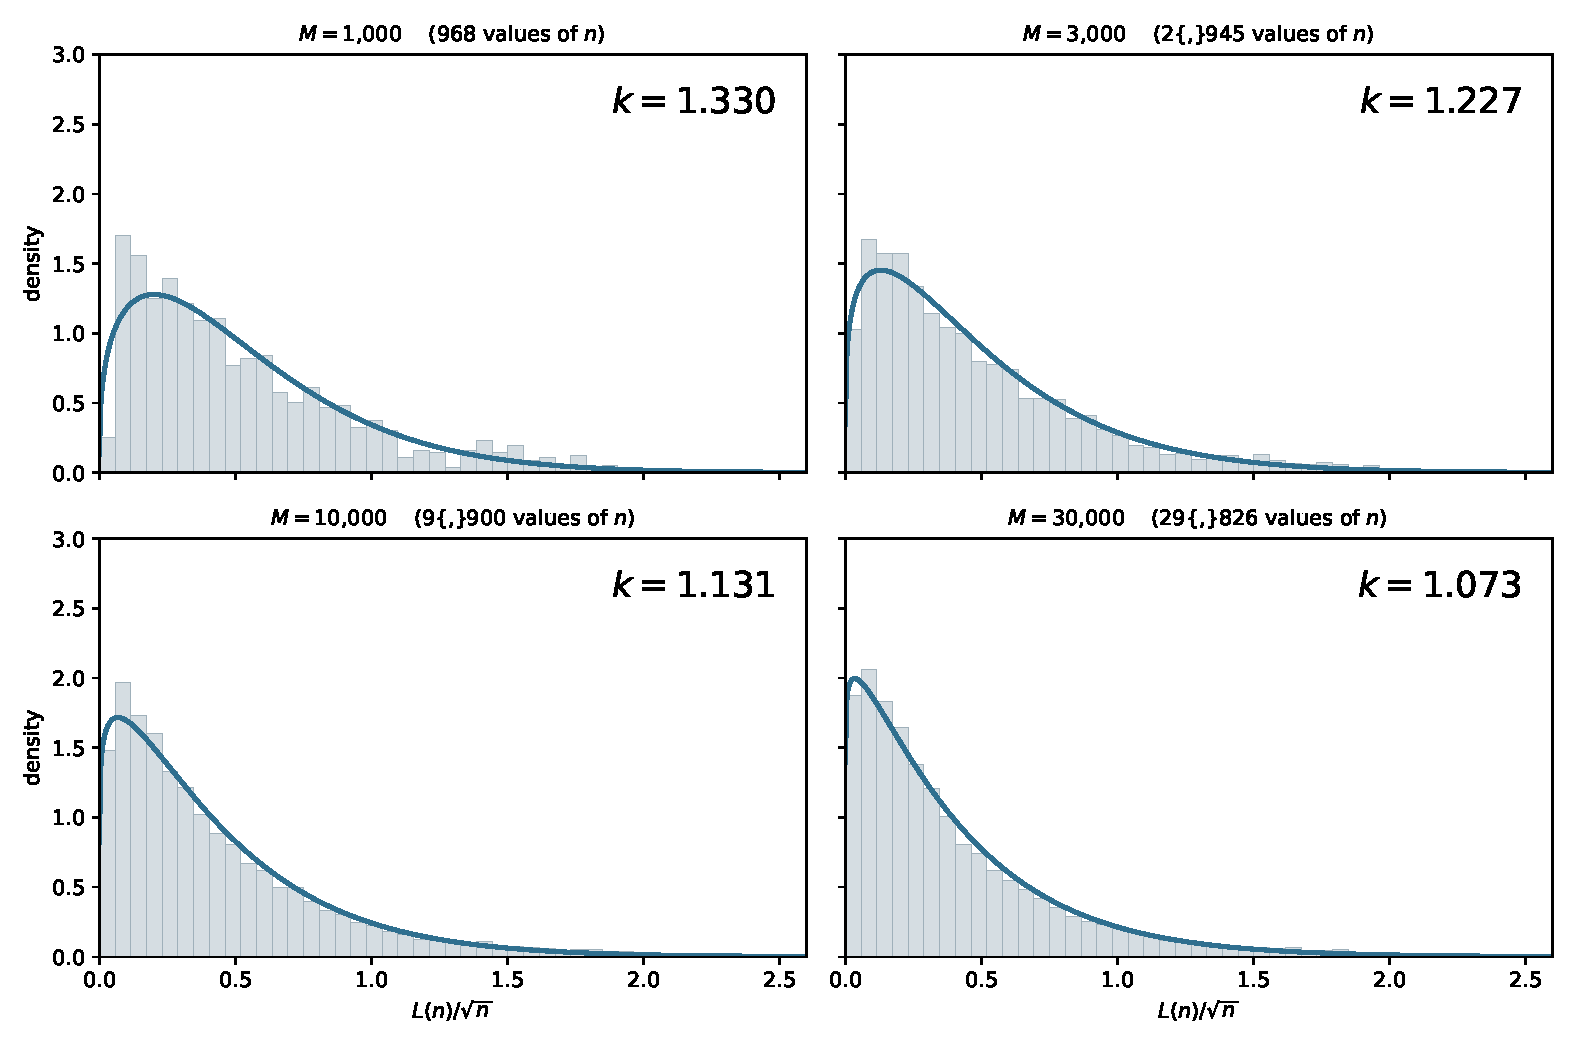
\includegraphics[width=\textwidth]{alogos-densities.pdf}
\end{center}

\begin{center}
\begin{tabular}{rrrr}
\toprule
$M$ & values of $n$ & $k$ & $\lambda$ \\
\midrule
$1{,}000$  & $968$    & $1.330$ & $0.574$ \\
$3{,}000$  & $2{,}945$ & $1.227$ & $0.514$ \\
$10{,}000$ & $9{,}900$ & $1.131$ & $0.457$ \\
$30{,}000$ & $29{,}826$ & $1.073$ & $0.418$ \\
\bottomrule
\end{tabular}
\end{center}

The four pictures look like one another. The fitted shape does not stay where it is.

\section{$k$ against $M$}

Repeating the fit at forty ceilings between $10^3$ and $10^6$:

\begin{center}
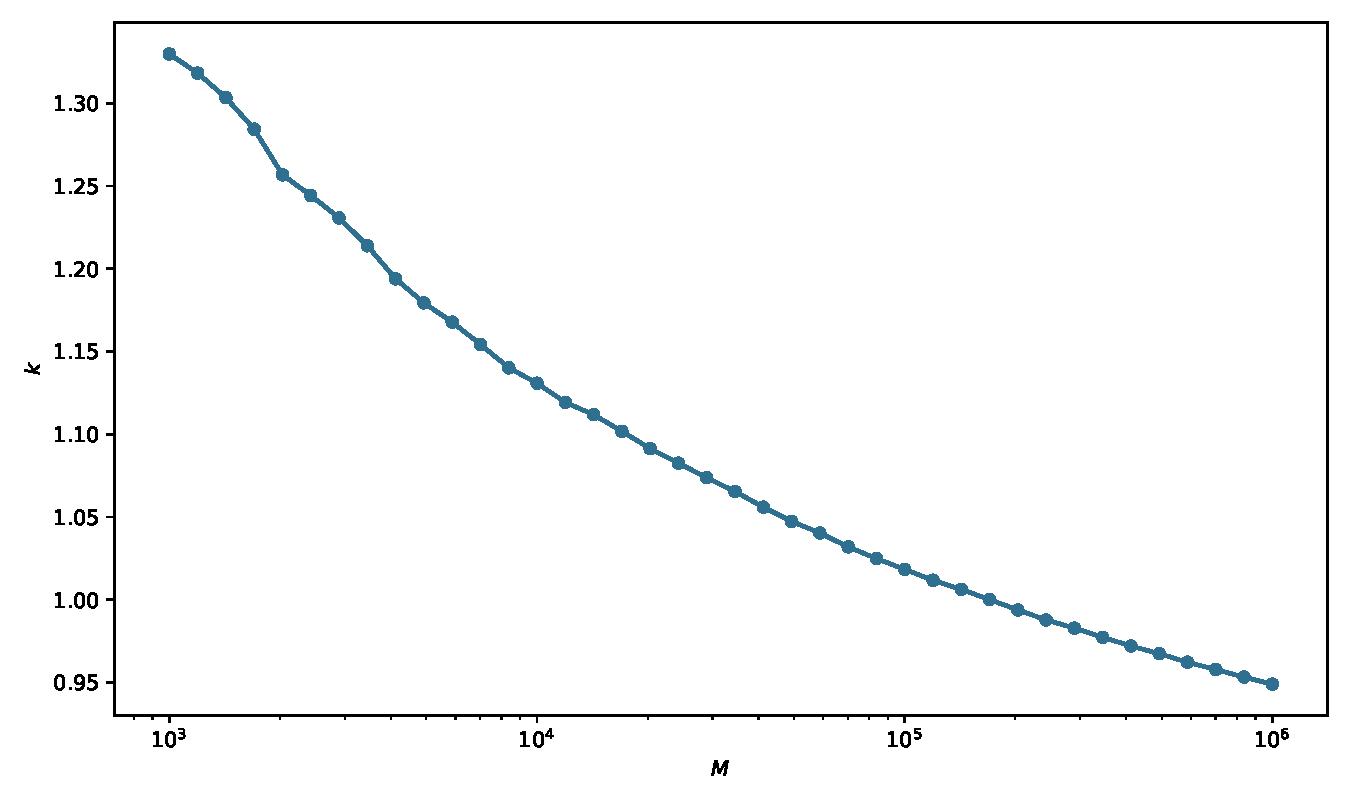
\includegraphics[width=\textwidth]{alogos-k-vs-M.pdf}
\end{center}

It runs from $1.330$ at $M = 1{,}000$ to $0.949$ at $M = 10^6$, downward throughout, and passes through $1$ on the way.

Two things are worth saying about that curve and nothing more should be read into it.

The first is that $k = 1$ is not an arbitrary level. It is the flat hazard, the memoryless case. So the curve crossing it means the qualitative description of the data reverses: below the crossing the fitted hazard rises with $t$, above it the hazard falls. A single sentence about the shape of this distribution is therefore true on one side and false on the other.

The second is that the descent is slowing. Measured decade by decade the slope is roughly $-0.093$, then $-0.049$, then $-0.030$, shrinking by a factor near $0.57$ each time. A quantity whose increments shrink geometrically may well converge, and several ways of extrapolating this one fit the measurements equally well and place the limit anywhere from $0.56$ to $0.86$. Which is to say the data establishes that $k$ is slowing down and establishes nothing whatever about where it stops.

\section{What this is}

$L(n)$ is determined. Every value was fixed before anyone computed it, there is nothing random in the construction, and each one can be produced exactly by the integer recurrence of Section 4. And the only available description of the collection is a statistical one, whose single most important parameter depends on how far you happened to count.

\end{document}
